\section{Measuring Tor's Current State of Resiliency to Hijack Attacks}

Because the Tor network is susceptible to network-level adversaries, we aim to quantify how much of the Tor network would be affected by a BGP prefix hijack.  First, we start by analyzing recent, publicized hijacks, and determine if they have affected the Tor network.  Then, we look at how to evaluate the Tor network in terms to susceptibility to hijack attacks.  The metrics used help enlighten the community about the state of the Tor network, in terms of how resilient the relays are to hijack attacks.  Additionally, this helps quantify how vulnerable the Tor network is to network-level adversaries in a novel way.  Specifically, we measure:

\begin{itemize}
\item Resiliency of the ASes that contain relays and compare the resiliency of ASes that contain more relays to those that contain few relays.
\item Impact of a BGP prefix hijack on the Tor network.
\item Probability of any given Tor relay being decieved by a BGP prefix hijack.
\end{itemize}

\subsection{Recent Hijacks in the Wild}

There have been a number of prefix hijack attacks in the past year.  We analyzed the BGP routing announcements and withdrawals from the known time-frames to find the prefixes that were hijacked and compared them to the list of Tor relay IP addresses at the time.  This shows us that prefix hijacks in the past year have affected Tor relays; it's also important to note that the analysis of publicized hijacks is not exhaustive.  There may be hijack attacks that were not publicized or not recorded, and could have affected the Tor network as well.  This analysis presents a lower-bound on the number of affected relays from two separate hijack attacks.  

From routing announcement logs, we have seen two attacks that have involved Tor relays: 

\begin{itemize}
\item On November 6th, 2015, AS9498 (BHARTI Airtel Ltd.) hijacked about 16,000 prefixes~\cite{indiahijack}.
\item On June 12th, 2015, AS4788 Telekom Malaysia started to announce about 179,000 of prefixes to Level3 (AS3549, the Global crossing AS)~\cite{malaysialeak}.
\end{itemize}

These are just incidents from the past year, but previous work has shown other, additional attacks that have affected the Tor network prior to 2015~\cite{sun2015raptor}.

\subsection{Resilience Methodology}

Previous work has tackled questions of AS resilience using simulations of the entire Internet \cite{lad2007understanding}.  We build off of this work by applying these metrics to the Tor network.  First, we measure the resiliency of Tor-related ASes to equal-length prefix hijack attacks.  To do so, we use an Internet topology~\cite{caida} to get all of the AS relationships, and construct and AS-level graph.  We identify the Tor-related ASes and simulate prefix hijacks on the graph. Specifically, our methodology consists of:

\begin{enumerate}
\item Construct an AS-level graph from an Internet topology.
\item Identify ASes that have at least one Tor relay.
\item Calculate the number of equally preferred paths from AS A to AS B, where AS B is a Tor-related AS.
\item Calculate the number of equally preferred paths from AS A to AS C, where AS C is the attacking (hijacking) AS.
\item Calculate resiliency using the equation in \cite{lad2007understanding}.
\end{enumerate}

We follow this methodology for every AS A $\neq$ a Tor-related AS, every AS C $\neq$ a Tor-related AS, and for every AS B $=$ Tor-related AS.

\cite{lad2007understanding} explains the probability of a node $v$ being deceived by a given false origin $a$ announcing a route that belongs to true origin $t$:

\[\beta(a,t,v) = \frac{p(v,a)}{p(v,a) + p(v,t)}\]

where $p(v,a)$ is the number of equally preferred paths from node $v$ to false origin $a$ and $p(v,t)$ is the number of equally preferred paths from node $v$ to true origin $t$.  Using this probability, the same researchers introduced the resiliency metric -- the resilience of a node $t$ is the fraction of nodes that believe the true origin $t$ given an arbitrary  hijack against $t$:

\[R(t) = \sum_{a \in N} \sum_{v \in N} \frac{\beta(t,a,v)}{(N-1)(N-2)}\]

where N is the total number of ASes.

%There is also space for metrics regarding specific relays' resiliency to BGP prefix hijack attacks, as well as metrics regarding BGP prefix interception attacks (AS- and relay-level).  

%  We also plan to specifically look at the resiliency of guard relays (as a group) as well as exit relays (as a group). 

\subsection{Resiliency Results and Values}

We obtained the list of Tor guard/exit relays from Tor consensus in December 2015 and retrieved their belonging ASes. Then, we downloaded the AS topology published by CAIDA in December 2015. We evaluated the resiliency of each of the ASes which contain Tor guard/exit relays based on the AS topology using the method in ~\cite{lad2007understanding}. 

The AS topology contains 52680 ASes, in which 612 ASes contain a total of 2548 Tor guard/exit relays. We simulated \emph{all} possible hijacking scenarios against each of the 612 ASes, totaling $52679 \times 612 = 32,239,548$ prefix hijacks. As stated in ~\cite{lad2007understanding}, the resiliency of an AS t is calculated by:
\begin{equation}
R(t) = \sum_{a \in N} \sum_{v \in N} \frac {\bar{\beta}(t,a,v)} {(N-1)(N-2)}
\end{equation}

in which $N$ is the set of all ASes, and $\bar{\beta}(t,a,v)$ is defined as:
\begin{equation}
\bar{\beta}(t,a,v) = \frac {p(v,t)} {p(v,t) + p(v,a)}
\end{equation}

in which $p(v,n)$ is the number of equally preferred paths from node $v$ to node $n$ given the routing policy and path lengths. Thus, we first calculate the resiliency of each Tor AS from each of the 52680 ASes as the \emph{source} AS as following, and then sum up the resulting resiliency $R$ to obtain the total resiliency for each of the Tor ASes. 
\\
\begin{algorithmic}
\Function{CalcResilience}{graph $G$, node $t$}
    \State \Call{CalcPathsFromNode}{$G,t$}
    \State $zeros(R)$
    \For{each reachable node $v$ from node $t$} 
    	\If{node $v$ contains Tor guard/exit relays}
		\State $n \gets $ number of less preferred nodes than node $v$
		\State $R[v] \gets n + (\bar{\beta}(v,a,t)$ $\forall$ equally preferred node a)
	\EndIf
    \EndFor
    \State \Return $R$
\EndFunction
\end{algorithmic}

Note that, the $\Call{CalcPathsFromNode}{G,t}$ step above requires AS-level path predictions. Previous works have shown that AS level paths are determined mainly based on two preferences~\cite{starov2015measuring}:

\begin{itemize}
\item Local Preference
\item Shortest Path
\end{itemize}

Further more, the AS paths should also have the \emph{valley free} property (citation here), meaning that  [summarize here about the property]. Thus, we use depth first search to traverse the graph from a given source node based on this property and the preferences. We first explore provider-customer paths, which are the most preferred; next, we explore one peer-to-peer path followed by a sequence of provider-customer paths, which are the next preferred; finally, we explore customer-provider paths followed by an optional peer-to-peer path and then followed by a sequence of provider-customer paths. Note that, nodes are explored in the most preferred to least preferred order, and those which are explored in the same step are equally preferred. This ordering will help the above resiliency calculation. 
\\
\begin{algorithmic}
\Function{CalcPathsFromNode}{graph $G$, node $t$}
	\State [to be filled]
\EndFunction
\end{algorithmic}

After calculating the resilience for each AS that contains at least one Tor relay, we can see that most ASes lie in the middle of the spectrum for resilience (as shown in Figure~\ref{fig:resilience_histogram}).

\begin{figure*}
\centering
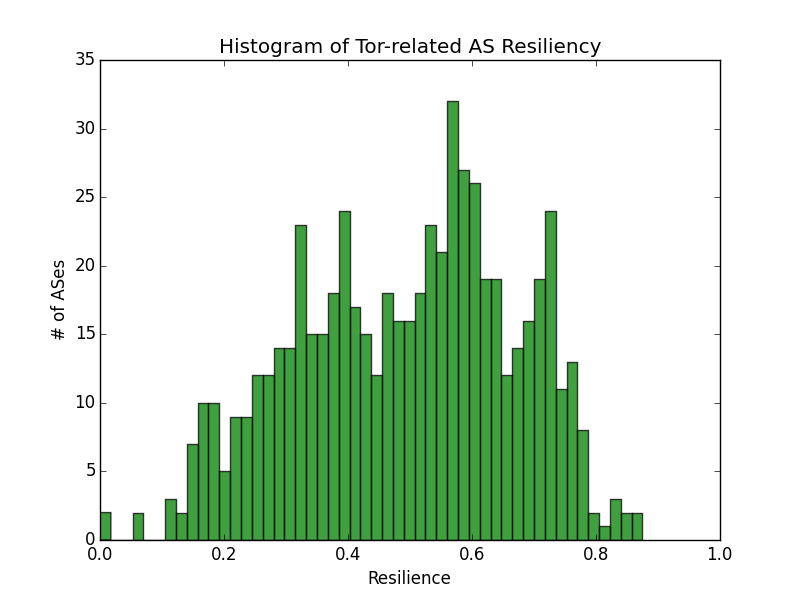
\includegraphics[width=.5\textwidth]{resilience_histogram}
\caption{A histogram of resilience values for all ASes that contain a Tor relay.}
\label{fig:resilience_histogram}
\end{figure*}

We then looked at which ASes had the most relays, and what their corresponding resilience is; ideally, ASes with more relays are also more resilient to hijack attacks.  Figure~\ref{fig:res_relays} shows the resilience value for an AS and the AS's corresponding number of relays.  

\begin{figure*}
\centering
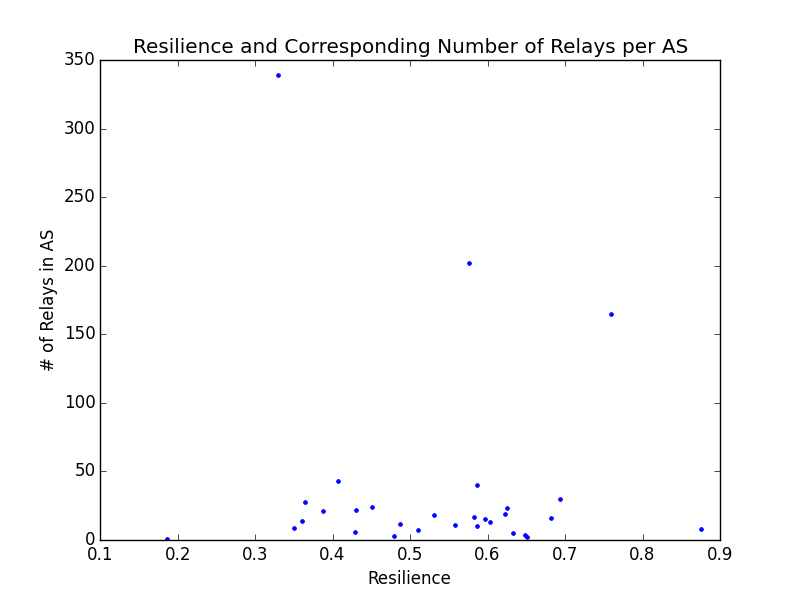
\includegraphics[width=.5\textwidth]{res_num_relays}
\caption{Resilience values for each AS and each AS's corresponding number of relays.}
\label{fig:res_relays}
\end{figure*}

We can see one outlier - AS16276 - which contains 339 relays; unfortunately, this AS also has a relatively low resilience against hijack attacks.  This motivates our proactive and reactive countermeasures against hijack attacks.
